% title section ================================================================
\begin{center}
    \large
    \textbf{Thesis Proposal: Using a Modified Point Net to \\ Generate 3D Bounding Box Proposals with Stereo Disparity Maps}\\
    \noindent \textbf{April-August 2019}\\
    \normalsize 
\end{center}

\begin{tabular}{ll}
    Student: & Kristian Gonzalez \\
    & Ravensburg-Weingarten University of Applied Sciences\\
    Supervisor: & Prof. Dr. Wolfgang Ertel \\
    & Ravensburg-Weingarten University of Applied Sciences\\
    Co-supervisor: & Prof. Dr. Stefan Elser\\
    & Ravensburg-Weingarten University of Applied Sciences\\
\end{tabular}

% body section =================================================================

\section{Introduction}
delme: things to talk about:
	a little about computer vision
	what are typical issues in field
	what is main problem?
	small sample of solution (to be intro'd later) \\
% %%%%%%%%%%%%%%%%%%%%%%%%%%%%%%%%%%%%%%
Computer vision is a field that has grown explosively in the last few years, very much in thanks to the utilization of convolutional neural networks, or CNN's, to accurately identify different kinds of information from raw image data. This capability has led to many different sub-fields of research, including 3D localization of objects using a variety of sensor setups. In having a branching set of possible sensor setups, a few questions naturally arise: how many sensors are needed to accurately locate objects, and how competitive are systems that do not directly take distance measurements to localize objects? 

In the field of autonomous driving, a ``typical" sensor system may include the following: forward facing camera, a complimentary second camera for stereo image generation, an IMU (inertial measurement unit), a lidar sensor (either a single sensor on the top or one at the front \& back of the vehicle), a forward-facing radar, and possibly other cameras facing various directions. 

%kjgnote: need examples: 
%kitti dataset: http://www.cvlibs.net/publications/Geiger2013IJRR.pdf
%apolloscape: https://arxiv.org/pdf/1803.06184.pdf
%Berkeley deep drive: https://bair.berkeley.edu/blog/2018/06/18/bdd-update/
%robotcar: https://robotcar-dataset.robots.ox.ac.uk/images/robotcar_ijrr.pdf
%(kjgnote: will omit others, i think the point gets across)

Because of this sensor complexity, this paper proposes to seek out a more streamlined approach by primarily utilizing stereo vision to create 3D bounding box proposals and estimates. The current norm in the field leans heavily towards using lidar-based networks (typically nets that use some combination of camera and lidar information), while this paper instead asks: can stereo disparity maps provide a competitive alternative by using methods adapted from lidar networks? It must be acknowledged at the start of this proposal that lidar sensors do typically provide more accurate distance measurements by virtue of directly measuring the environment, but not without downsides. Lidar technology is typically expensive (although this price is decreasing), and has difficulty with reflective surfaces. Therefore, the aim of this paper is not to obtain better 3D object detection than lidar, but to demonstrate stereo vision's competitiveness. 

To that end, this paper proposes a novel method of using stereo disparity maps to localize objects. A modified stereo depth estimation network, Pyramid Stereo Matching Network (PSMnet), will be used to generate a stereo image, which will then be projected to 3D point space and fed into a well-known point network, Frustum Point Net (FPnet).


\section{Related Work}
delme: things to talk about:
	existing 3D bounding box networks that use stereo
	different kinds of stereo networks / methods
	different 3D bounding box networks (non-stereo) \\
% %%%%%%%%%%%%%%%%%%%%%%%%%%%%%%%%%%%%%%

\subsection{Convolutional Networks Using Point Clouds}
A variety of networks exist that estimate 3-dimensionsal bounding boxes, including Frustum PointNet, which is to be modified in this paper. FPnet takes a three step approach, which includes: ``traditional" 2D object detection, 3D segmentation, and amodal estimation. This is demonstrated below in figure xx, reproduced from the original paper.
\begin{figure}[h] % h = "approx here", {h,t,b}
    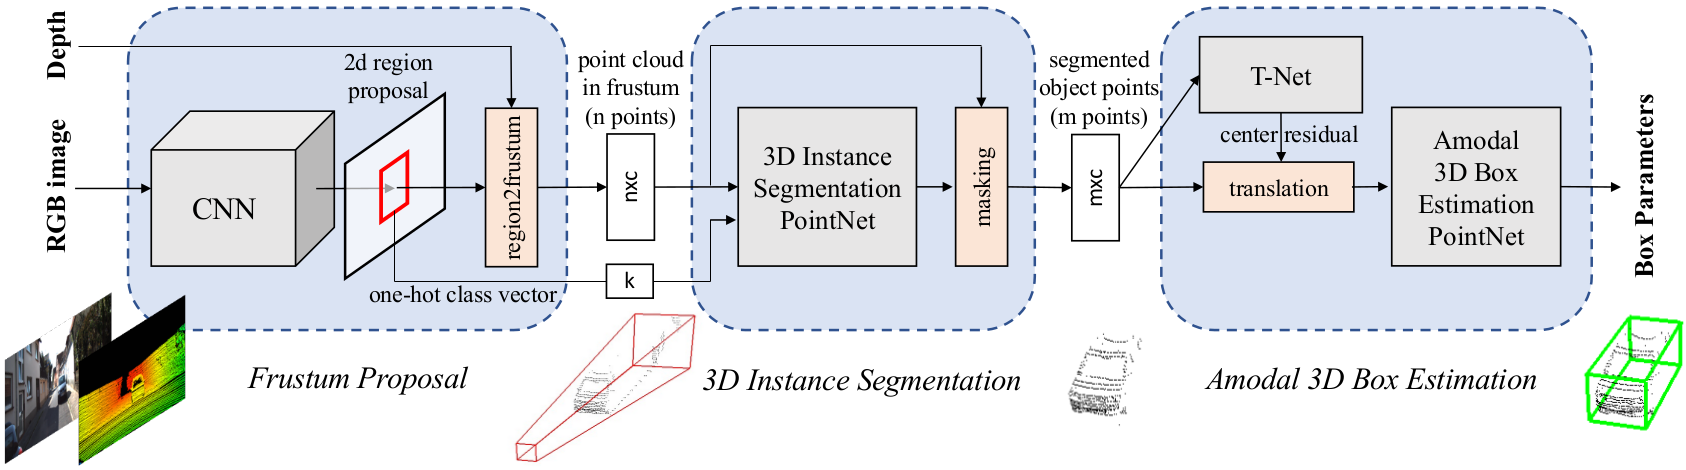
\includegraphics[width=1\textwidth]{m/fpnet_steps.png}
    \caption{Reproduced image of general FPnet steps. First, 2D object detection locates an image and creates a "frustum" (or cone) of the valid lidar point cloud. Next, this reduced set of points segmented in the 3D space, by removing the fore- and background points. Finally, an estimate of the remaining points is made about the object's size and orientation to generate a bounding box.}
% \label{figure-parking}
\end{figure}


The first point net to successfully implement this approach was the aptly-named "Pointnet" \cite{qi2017pointnet}, which focused on working with point cloud data in its native format, rather than transform the data to 3D voxel grids or views. This approach provides some clear advantages over networks like Voxnet \cite{maturana2015voxnet}, which relies on creating a three-dimensional occupancy grid requiring a reference frame and given resolution. Though creating volumetric or 3D CNN's created an initial approach, they are limited by data sparsity and computation cost. By contrast, the original Pointnet and subsequent FPnet are designed to work with a point cloud's inherent properties, paraphrased from \cite{qi2017pointnet}: 
\begin{itemize} \itemsep=-0.5em
    \item Unordered: point clouds are essentially an undordered set of vectors containing \textit{x,y,z} coordinates, among other information.
    \item Point interaction: because the points come from euclidean space, neighboring points form a meaningful group, so any network must be able to represent the "local structures" of a subset of points.
    \item Invariance under transformation: some simple transformations, such as rotation, translation, or scaling, do not change the inherent category the object belongs to, such as a car or plane.
\end{itemize}

Using multiple views is another approach taken to tackle point cloud data. In practice, multiview CNN's project 3D point clouds onto 2D planes, then apply 2D CNN's for classification. However, this rapidly increases in copmlexity when extending the usage to understanding or shape completion. 

\subsection{Using CNN's to Generate Stereo Disparity Maps}
Creating a dispartity map by use of two cameras, or stereo matching,has its roots in finding a matching pixel between two cameras to understand its distance away from the cameras by use of epipolar geometry. Typically, an image similar to figure xx (reproduced from Hamzah and Ibrahim \cite{hamzah_literature_2016}) below is used to illustrate this. 

\begin{figure}[h] % h = "approx here", {h,t,b}
    \centering
    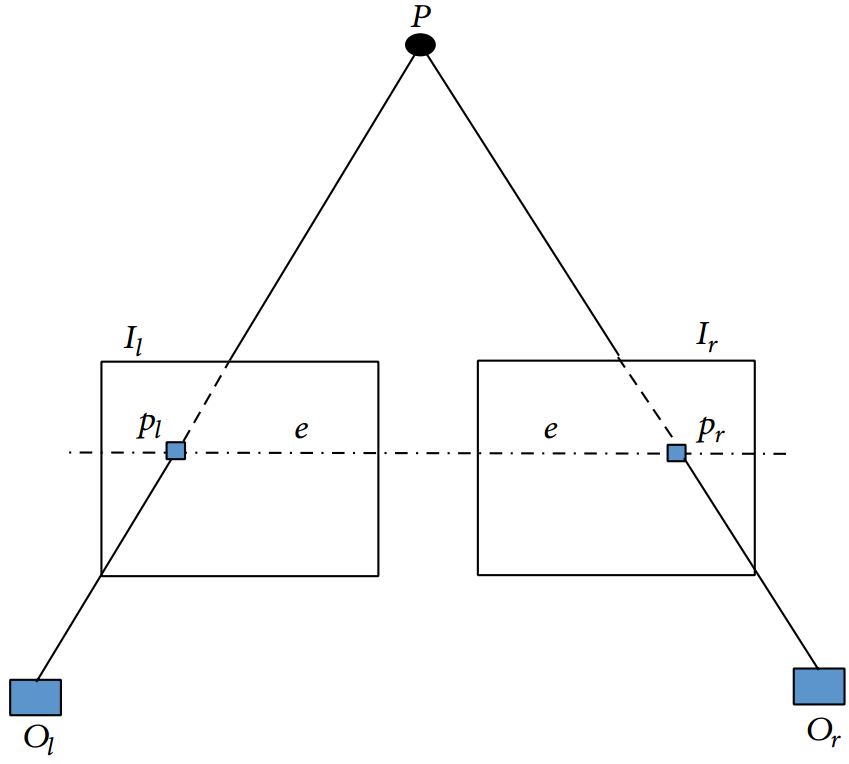
\includegraphics[width=0.375\textwidth]{m/stereo_parallax.png}
    \caption{Using trigonometry, a target at point P can be located on two image planes at their local points and estimated at a certain distance from the sensors.}
    % \label{figure-parking}
\end{figure}

Creating a disparity map has its roots in mathematically rigorous approaches, typically starting with trigonometry and parallax to explain how distance may be estimated from two cameras separated by a known distance. This gives rise to the term stereo matching. Ibraim and Hamzah \cite{hamzah_literature_2016} present a comprehensive but not exhaustive survey on existing algorithms, many of which used only a CPU for their calculations. However, as also stated, the "number of calculations required increases with an increasing number of pixels", making the matching problem computationally complex. 

\subsection{Using Stereo Disparity Maps and CNN's for 3D Object Detection}


\section{Proposed Solution}
delme: things to talk about: 
	what is your general approach
	how is each part to be prepared
	how will results be verified?
	what are your expected risks?
	what is expected timeline of project \\
% %%%%%%%%%%%%%%%%%%%%%%%%%%%%%%%%%%%%%%
TextHere








% ==============================================================================
% ANYTHING PAST THIS IS MERELY TEMPORARY, TO BE DELETED ========================
% ==============================================================================











%\section{Introduction}
%delme:
%Computer vision is a field that has grown explosively in the last few years, very much in thanks to the utilization of Convolutional Neural Networks, or CNN's, to accurately identify different kinds of information from raw image data. This capability has led to many different subfields of research, including 3D localization of objects using a variety of sensor setups. To that end, a few questions naturally arise: how many sensors are needed to accurately locate objects, and what trade-offs exist for using certain sensors over others, such as stereo vision instead of the more expensive lidar systems? 
%
%This paper proposes to seek out an alternative approach to lidar-based 3D object detection with the purpose of improving the state of the art in stereo-based object detection. It must be acknowledged at the start of this proposal that lidar sensors do typically provide more accurate distance measurements, but not without downsides. Lidar sensors are active, and thus must also emit a laser in order to determine distance. This is a source of both higher cost as well as potential interference if many autonomous systems were to use them at once, such as in autonomous driving. Therefore, the aim of this paper is not to obtain better detection than lidar, but to demonstrate stereo vision's competitiveness. 
%
%
%To that end, a paper is proposed to seek out a comparison between two specific sensor setups. The first sensor setup would use only camera data, and a derived stereo disparity image, to detect and localize the desired object of interest, specifically cars. The second sensor setup would use a single camera and a single lidar to perform the same task. The nature of the detection required would be a 3D bounding box, expressed as a box with real-world distances to describe an object's relative x, y, and z coordinates as well as its height, width, and length. The dataset that would be used for this task is not yet confirmed, but is currently one out of several possibilities, described below. Each of these possible datasets will be expanded upon below, describing their merits and drawbacks.
%
%
%rawtext: \\
%so, have met with prof elser and ertel on 190307. after some discussion and open talk, it seems like there's some good ideas to really make a worthy thesis: 
%
%1. take frustum pointnet (fpnet) and the kitti dataset
%2. take pyramid stereo matching net (psmnet) and train it to properly generate stereo images from 2 rgb images
%3. modify frustum pointnet to accept stereo images from pretrained network (so perhaps a 2-step training process)
%4. have frustum pointnet train on new incoming data
%
%so, what's the problem being addressed in this project? 
%in the sota approach, 3d bounding boxes are created by using lidar. however, lidar is expensive and relatively complex
%
%what's the solution in this project? 
%using an approach originally developed for lidar, fpointnet, will modify network to use stereo data and then evaluate its performance
%
%what's the hypothesis of this project?
%the modified fpnet will perform better than current stereo-based approaches, although perhaps still some fraction of the capability of the original network, but using only 2 cameras rather than camera \& lidar.
%
%
%
%
%% ==============================================================================
%\section{Literature Search Questions}
%There are multiple questions to answer regarding what is possible in this project. To that end, a literature search is underway to answer:
%
%\begin{itemize} \itemsep=-0.5em
%\item What is the state of the art in current stereo vision-based object detection? % kjg done
%\item What is the state of the art in current camera/lidar-based object detection?  % in progress
%\item What is the method that will be taken to improve stereo detection? % in progress
%\item What dataset meets the required criteria for usage in this project?			% in progress
%\item How are 3D bounding boxes evaluated, and what standard is used to obtain a score, such as precision, recall, and average precision? % in progress
%\end{itemize}
%
%% ==============================================================================
%\subsection{State of the Art: Stereo-Based Object Detection}
%To know the state of the art (SOTA) of stereo-based object detection, one may look at various benchmarks that use a single, common dataset to compare multiple networks and algorithms. The well-known Middlebury \cite{scharstein2014high,middlebury_leaderboard} dataset is a common benchmark, as well as the KITTI \cite{geiger_are_2012,kitti_leaderboard} 2015 Stereo benchmark. Additionally, there are even some aggregate lists, including the 2018 Robust Vision Challenge \cite{rvc_leaderboard} leaderboard. Looking at the aggregated Robust Vision Challenge leaderboard, last updated in December 2018, two top-performing networks are iResNet, holding 1st place, as well as PSMNet, in 4th place. What also makes these two stereo networks special is that both have publicly available repositories. Furthermore, PSMNet, or Pyramid Stereo-Matching Network, has simpler and fewer dependencies than iResNet. Lastly, PSMNet is (as of this writing) in the top 10 of the current KITTI 2015 leaderboard. Therefore, this project will use PSMNet's method to generate and use stereo disparity maps. 
%
%\subsection{State of the Art: Camera/Lidar-Based Object Detection}
%TextHere 
%kjgnote: here you should talk abot frustum net as well as other approaches. 
%
%\subsection{Proposed Method to Improve Stereo-Based Object Detection}
%TextHere
%
%
%\subsection{Valid Datasets, and the Most Qualified to be Used}
%In order to perform good object detection, a dataset must exist that meets the project needs. In this project, the various requirements are listed below. \\
%
%A usable dataset for this project must have: 
%\begin{itemize} \itemsep=-0.5em
%    \item RGB (red/green/blue, 3-channel) images
%    \item Stereo vision disparity maps, or the ability to generate them
%    \item Man-made objects as the class of interest, e.g. cars
%    \item 3D bounding boxes for object localization
%    \item Data collected in an outside setting
%    \item OPTIONAL: lidar data containing the class of interest (for future comparison with other methods).
%\end{itemize}
%
%Based on these criteria, some datasets may be valid or invalid, and merit investigation. The following datasets all meet the necessary requirements, and some also contain the optional requirement.
%\begin{itemize} \itemsep=-0.5em
%    \item The KITTI dataset (3D detection task)
%    \item Oxford RobotCar dataset (3D detection task)
%    \item Berkeley DeepDrive Dataset
%    \item (TBD)
%\end{itemize}
%
%
%\subsection{3D Bounding Box Evaluation}
%In order to properly evaluate the detections of the network's 3D bounding boxes, the well known methods of evaluating 2D bounding boxes must be adapted. This has already been investigated by and accomplished by (need source) those at the kitti dataset. For the KITTI benchmark 3D detection challenge, an evaluation method was developed and proposed by xx. Thus, this method will be followed to evaluate and compare performance of the network. 
%
%\section{Project Schedule / Timeline}
%In order to meet all requirements while also satisfying educational program requirements, a proposed timeline is provided below. Notable dates here include the official start of the thesis, the final date of the thesis, including presentation and document turn-in.
%
%% kjgnote: "makebox" used in order to make an oversized-but-still-centered figure
%\begin{figure}[h] % ahh, h = "approx here", t = "top of page", b = "bottom of pg"
%    \makebox[\textwidth][c]{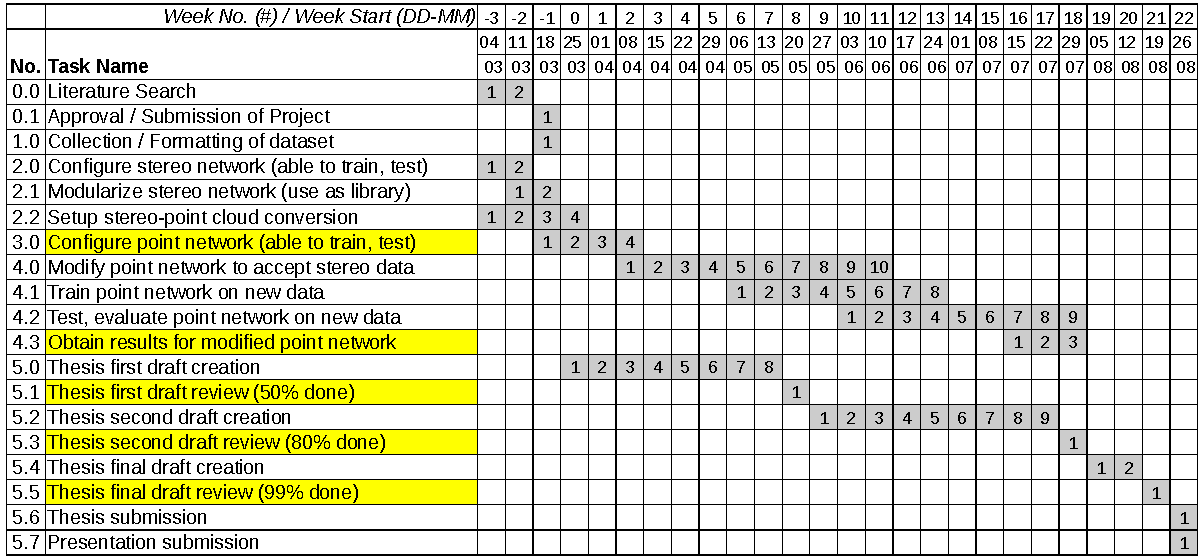
\includegraphics[scale=.6]{m/proposed_timeline.pdf}}
%    \caption{Proposed schedule of paper. Highlighted tasks are critical milestones. Numbers inside of gray cells indicate the number of weeks each individual task lasts.}
%% \label{figure-parking}
%\end{figure}


